\chapter{Frames}\label{ch:frames}
A coordinate system is a reference framework that defines the position in either two- or three-dimensional space. In this chapter, the relationship between the coordinate system for the world and for the Cobra robot will be taken into account. In figure \ref{fig:sub-transformation}, it is shown that the world coordinate is rotated and translated with respect to the robot frame. 
%\begin{figure}[hb]
%  \centering
%  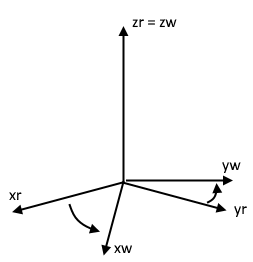
\includegraphics[width=3.5in]{figures/coordrobottoworld.png}
%  \caption[Checkerboard and coordinate with robot to world] {Checkboard and coordinate with robot to world}
%  \label{fig:check_coordrobottoworld}
%\end{figure}

\begin{figure}[hb]
\hfill
\subfigure[From robot to world frame]{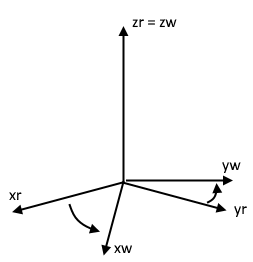
\includegraphics[width=5cm]{figures/coordrobottoworld.png}\label{fig:sub-transformation}}
\hfill
\subfigure[Checkerboard]{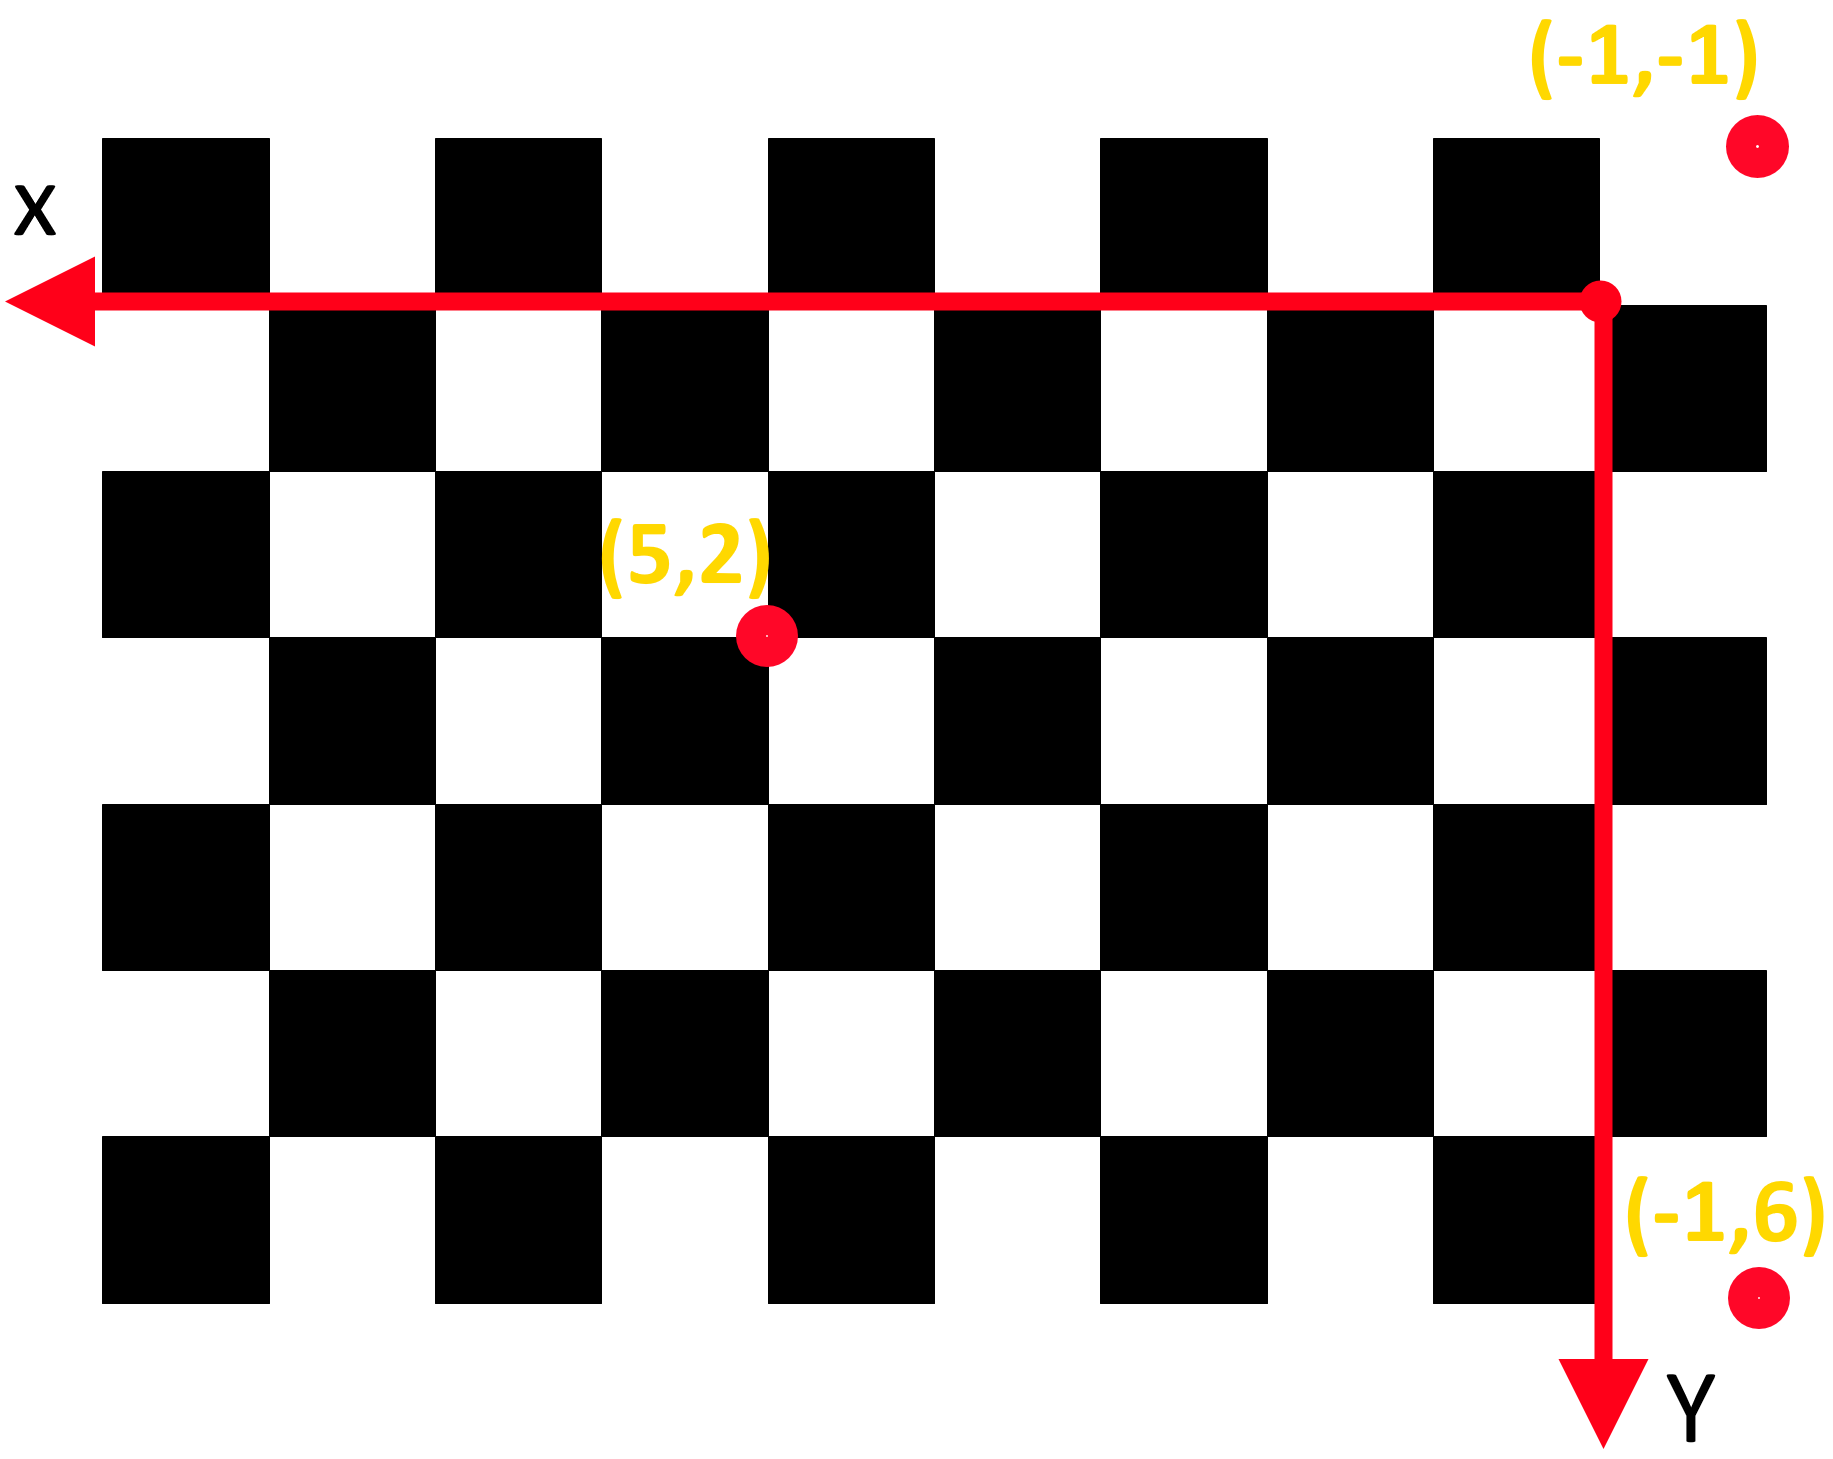
\includegraphics[width=5cm]{figures/pattern.png}\label{fig:sub-checkerboard}}
\hfill
\caption{Title for both}
\end{figure}

The following equation shows the relationship between the robot frame and the world frame. It is assumed that the z axis is on the same axis in both robot and world coordinate, because the blocks lay on the XY plane. Therefore the following equation can we written as: 
\begin{align*}
\begin{bmatrix}
x_r \\
y_r \\
z_r \\
1 
\end{bmatrix}
= \underbrace{\begin{bmatrix}
a & b & x & c \\
d & e & x & f \\
g & h & x & i 
\end{bmatrix}}_{\text{R | T}}
\begin{bmatrix}
x_w \\
y_w \\
z_w\\
1 
\end{bmatrix}
= \underbrace{\begin{bmatrix}
a & b & c \\
d & e & f \\
g & h & i 
\end{bmatrix}}_{\text{    R   | T}}
\begin{bmatrix}
x_w \\
y_w \\
1 
\end{bmatrix}
\label{eq:world_to_robot}
\end{align*}


In order to find the coordinates $(x_r,y_r,z_r)$ in the robot frame, the matrix [R | T] and the coordinates in the world frame $(x_w,y_w,z_w)$ must be known. However, in this situation, only  the coordinates in the world frame were known, as calculated in the former chapter by means of the \textit{P} matrix. So, in order to find the robot coordinates in equation \ref{eq:world_to_robot}, the matrix [R | T] needs to be calculated. An easy way to find the solution of this issue would be to solve the [R | T] matrix as a system of equations. So that, if one point is known in the robot frame and in the world one, we will have three equations with nine unknowns as described in equations \ref{eq:system_of_equations1} to \ref{eq:system_of_equations2}.
 
\begin{align}
\label{eq:system_of_equations1}
x_r &= a\cdot x_w + b\cdot x_w + c \\
y_r &= d\cdot x_w + e\cdot x_w + f \\
1 &= g\cdot x_w + h\cdot x_w + i
\label{eq:system_of_equations2}
\end{align}
As a consequence, two more points are required to find 6 more equations to complete the system. 

The next step is to manually drive the robot to three different positions using the checkerboard as a reference, as shown in figure \ref{fig:sub-checkerboard}. The measured points are presented in the "REF TABLE" along with the final system of equations.

\begin{table}[h]
\begin{tabular}{| c | c | c | c |}
\hline
   & Point 1 & Point 2 & Point 3 \\
   \hline
  World & 28*[-1\quad -1] & 28*[-1\quad 6] & 28*[5\quad 2] \\
  Robot & [239.484\quad 198.714] & [233.953\quad 398.995]   & [408.578\quad 287.651] \\
  \hline
\end{tabular}
\end{table}

\begin{align*} 
p_1(x_r) &= a\cdot p_1(x_w) + b\cdot p_1(y_w) + c \\
p_1(y_r) &= d\cdot p_1(x_w) + e\cdot p_1(y_w) + f \\
1 &= g\cdot p_1(x_w) + h\cdot p_1(y_w) + k \\
p_2(x_r) &= a\cdot p_2(x_w) + b\cdot p_2(y_w) + c\\
p_2(y_r) &= d\cdot p_2(x_w) + e\cdot p_2(y_w) + f \\
1 &= g\cdot p_2(x_w) + h\cdot p_2(y_w) + k \\
p_3(x_r) &= a\cdot p_3(x_w) + b\cdot p_3(y_w) + c \\
p_3(y_r) &= d\cdot p_3(x_w) + e\cdot p_3(y_w) + f \\
1 &= g\cdot p_3(x_w) + h\cdot p_3(y_w) + k
\end{align*}
Finally, the relationship between the robot and world frame can be described by the following equation: 
\begin{align*}
\begin{bmatrix}
x_r \\
y_r \\
1 
\end{bmatrix}
= \underbrace{\begin{bmatrix}
1.0206 & -0.0282 & 267.2713 \\
0.0185 & 1.0218 & 227.8426 \\
0 & 0 & 1.0000 
\end{bmatrix}}_{\text{R | T}}
\begin{bmatrix}
x_w \\
y_w \\
1 
\end{bmatrix}
\end{align*}

